\documentclass[a4paper]{article}

\usepackage[english]{babel}
\usepackage[utf8]{inputenc}
\usepackage{amsmath}
\usepackage{verbatim}
\usepackage{graphicx}
\usepackage{hyperref}
\usepackage[colorinlistoftodos]{todonotes}
\usepackage{float}
\usepackage{geometry}

\title{STLDD - Software Top Level Design Document}
\author{Team 2}

\begin{document}
	\begin{titlepage}
		\newgeometry{left=2cm,top=1cm,right=2cm}
		\newcommand{\HRule}{\rule{\linewidth}{0.5mm}}
		
		\begin{minipage}{0.5\textwidth}
			\begin{flushleft} % Responsible persons, write on separate lines
				\textit{Responsible for this document:}\\
				Oscar Axelsson \\
				Daniel Olsson \\
				Jacob Mejvik
			\end{flushleft}
		\end{minipage}
		~
		\begin{minipage}{0.4\textwidth}
			\begin{flushright}
				PUSS154214
				\today
			\end{flushright}
		\end{minipage}\\[3cm]
		
		\centering
		\textsc{\LARGE Team 2}\\[0.5cm]
		
		\HRule \\[0.4cm]
		{ \huge \bfseries Software Top Level Design Document}\\[0.4cm] % Title of your document
		\HRule \\[1.5cm]
		
		\vfill
		\begin{flushleft}
			%Authors, write on separate lines
			\textit{Authors of this document:}\\
			Jacob Mejvik \\
			Oscar Axelsson \\
			Daniel Olsson
		\end{flushleft}
		
	\end{titlepage}
	\pagenumbering{gobble}
	\setcounter{tocdepth}{2}
	
	\begin{center}
		\textit{\large Version History}
		
		\begin{tabular}{ | l | l | l | p{5cm} |}
			\hline
			\textbf{Version} 	& \textbf{Date} 	& \textbf{Responsible} 	& \textbf{Description} 		\\ \hline
			1.0				 	& 230915 			& DO, JM, OA			&  Baseline. 				\\ \hline
		\end{tabular}
	\end{center}
	
	
	\tableofcontents
	\newpage
	\pagenumbering{arabic}
	
	\section{Introduction}
	This document describes the top level design of the Lamp Controller Application, which is an application used to control a light bulb and a sensor device. The application is developed as a project within the course "Software Development for Large Systems - ETSN05" at LTH.
	
	\section{Reference Documents}
	SRS - Software Requirements Specification, PUSS154212 v1.1
	
	
	\section{Overview}
	The main purpose of the Lamp Controller Application is to provide an interface used to control a light bulb and a sensor device from an MVD via a REST API provided by the backend. The application will provide three different views to detect and control the different devices.
	
	\subsection{Controller Application}
	\begin{itemize}
		\item{\textbf{BaseActivity:}} 
		The BaseActivity for the application that will connect the Activities with the NetworkManager.
		\item{\textbf{MyDeviceActivity:}} 
		Is the start screen of the application. Will contain a ListView and has methods for detecting devices and control a device that was selected from the ListView.
		\item{\textbf{DeviceListAdapter:}} 
		Adapter that handles the list in MyDevicesActivity, the ListView can display any data provided that it is wrapped in a ListAdapter. 
		\item{\textbf{Device:}} 
		Is an Abstract class that controlls the two devices we are handling. 
		\item{\textbf{SensorDevice:}} 
		Class containing the SensorDevice information.
		\item{\textbf{LightBulb:}}
		Class containing the LightBulb information.
		\item{\textbf{DeviceActivity:}} 
		Is an abstract class that holds the shared parameters deviceName and macAddress. It also contains an abstract method toggle that controls the on/off switch on the devices.
		\item{\textbf{SensorDeviceActivity:}} 
		Is the controller in the interaction with the user in the SensorDevice View. Controls the TextView fields and the buttons that will retrieve information regarding the sensors from NetworkManager.
		\item{\textbf{LightBulbActivity:}} 
		Is the controller in the interaction with the user in the LightBulb View. Controls the EditText fields and the buttons that will retrieve and send information from/to the NetworkManager.
		
		\item{\textbf{NetworkManager:}} 
		Handles all the communication with the API. The different methods for controlling both receiving and setting data.
		\item{\textbf{SensorValues:}} 
		A class for the information of the different sensors.
		
	\end{itemize}

	\subsection{Packages}
	\begin{itemize}
		\item Network
		\item Activity
		\item Adapter
		\item Model
		\item Sensor
	\end{itemize}

\subsection{UML diagram}
	\begin{figure}[H]
    \centering
    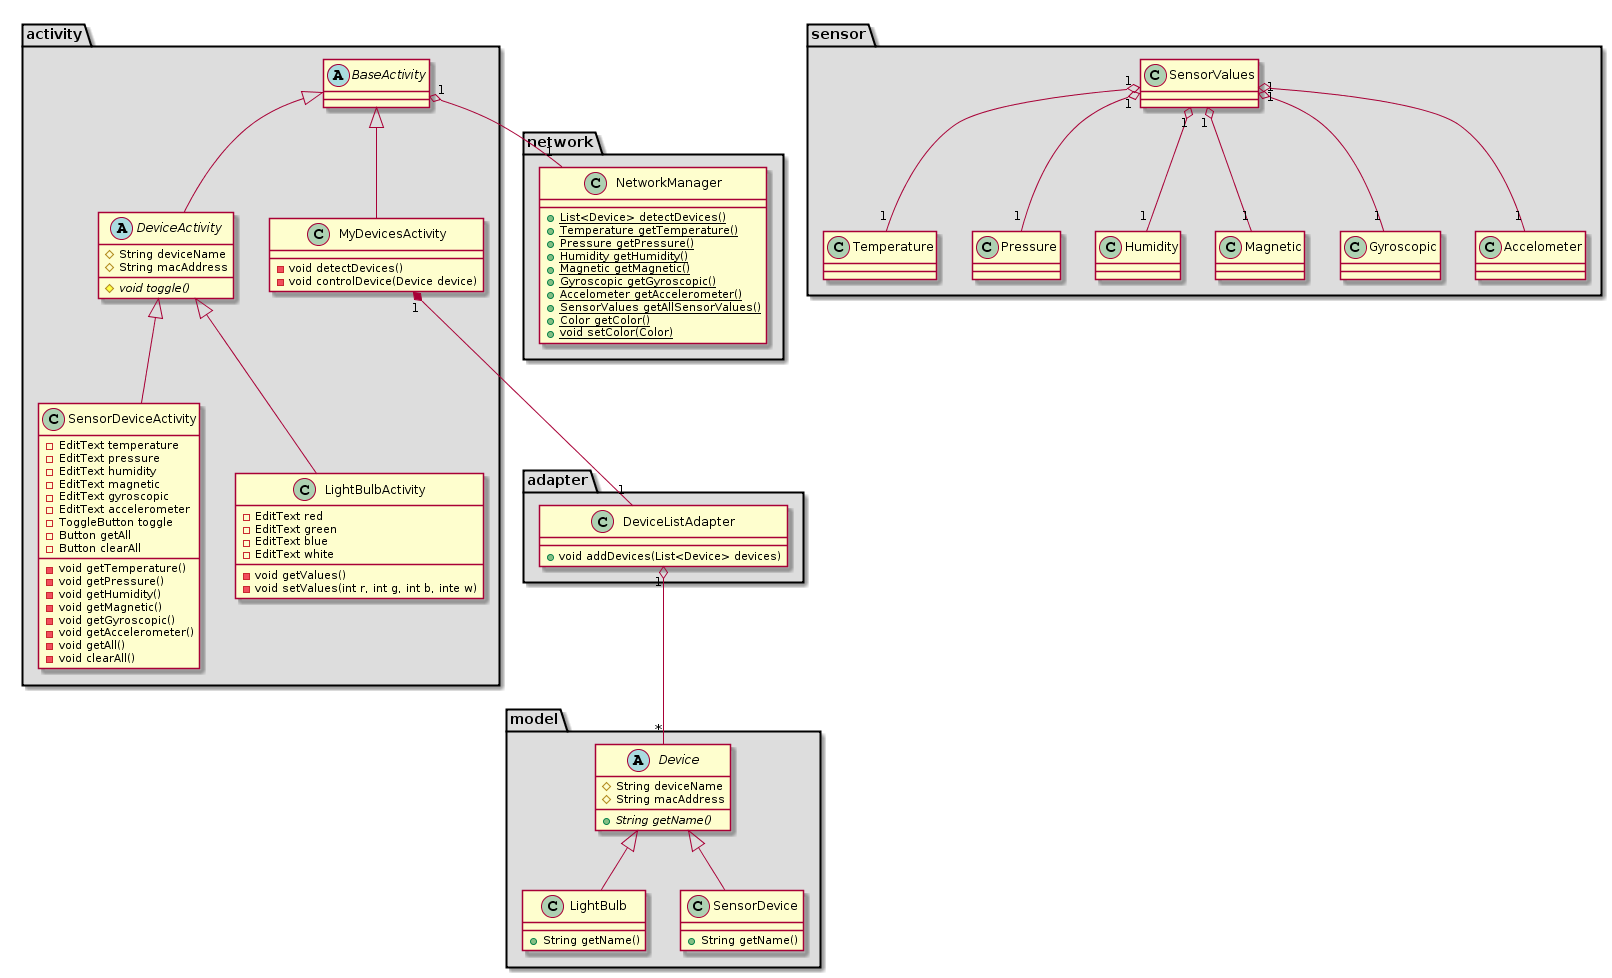
\includegraphics[width=0.4\textwidth]{class_diagram.png}
    \caption{The design of the system.}
    \label{fig:seq}
\end{figure}

	
	\subsection{Sequence diagrams}
	
	\begin{figure}[H]
    \centering
    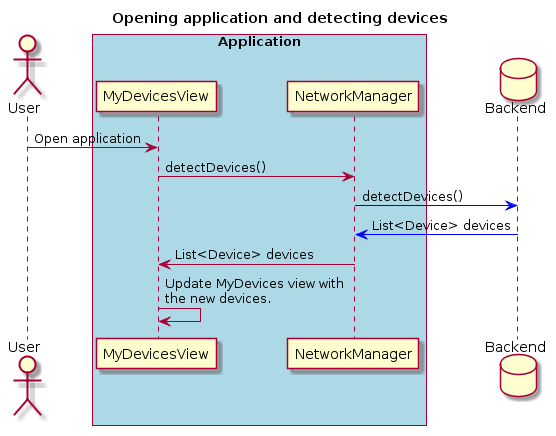
\includegraphics[width=0.4\textwidth]{seq.png}
    \caption{Detecting devices with the user located in MyDeviceView.}
    \label{fig:seq}
\end{figure}

\begin{figure}[H]
    \centering
    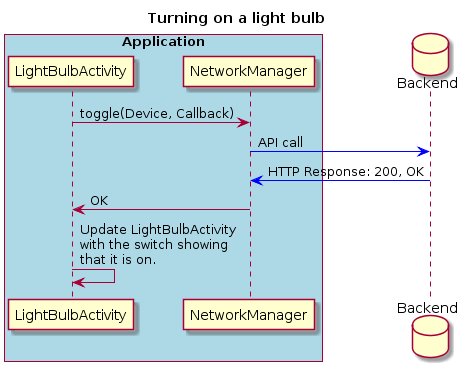
\includegraphics[width=0.4\textwidth]{seq1.png}
    \caption{Switch on the Light bulb with the user located in the LightbulbView.}
    \label{fig:seq1}
\end{figure}

\begin{figure}[H]
    \centering
    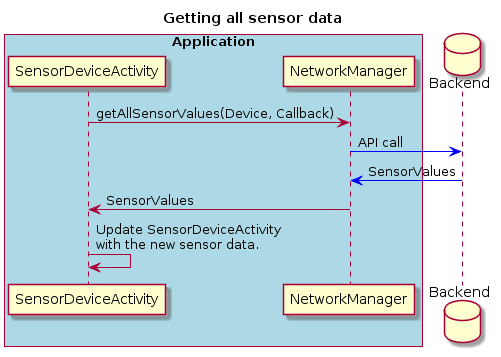
\includegraphics[width=0.4\textwidth]{seq2.png}
    \caption{Get all sensordata with the user located in the SensorDeviceView.}
    \label{fig:seq2}
\end{figure}

\begin{figure}[H]
    \centering
    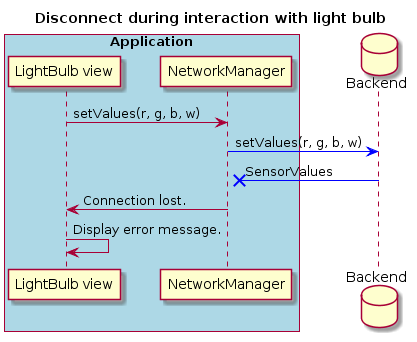
\includegraphics[width=0.4\textwidth]{seq3.png}
    \caption{Switch on Light bulb with the user located in the LightbulbView and the backend is unresponsive.}
    \label{fig:seq3}
\end{figure}
	
\end{document}